\subsection{Overall Capabilities}
\label{sec:capabilities}

\subsubsection{Hierarchical approach with multiple models}

``Hierarchical approach with multiple models, going from low fidelity
(eg.\  laminar fluid and fluid-kinetic runs in 2D) to medium fidelity (eg.\ 
fluid runs with neutrals and turbulence  multispecies, but with reduced number
of species) and high fidelity (eg.\  full kinetic or hybrid kinetic/fluid runs
with turbulence and multispecies approach).''

The plan is for \nep\ to provide a framework for solving relevant physics
models, and a user-friendly Domain-Specific Language (DSL) for doing this.
This allows UKAEA to develop its own physics models in a manner significantly
independent of \nep\ development and code distribution, see \Fig{proxyflow2}.
This is the same approach as currently used by UKAEA for BOUT++,
where UKAEA has ownership of physics models in the STORM software, while other organisations have
ownership of the BOUT++ framework.

Project \nep \ intends to provide a suite of examples of physics models as part of the code
distribution.
As addressed in \S\ref{sec:physics_model}, there is also development of a
physics model under \nep\ that could be adaptive, displaying a range
of fidelities within different regions of the domain during a single
simulation.

\begin{figure}
\centerline{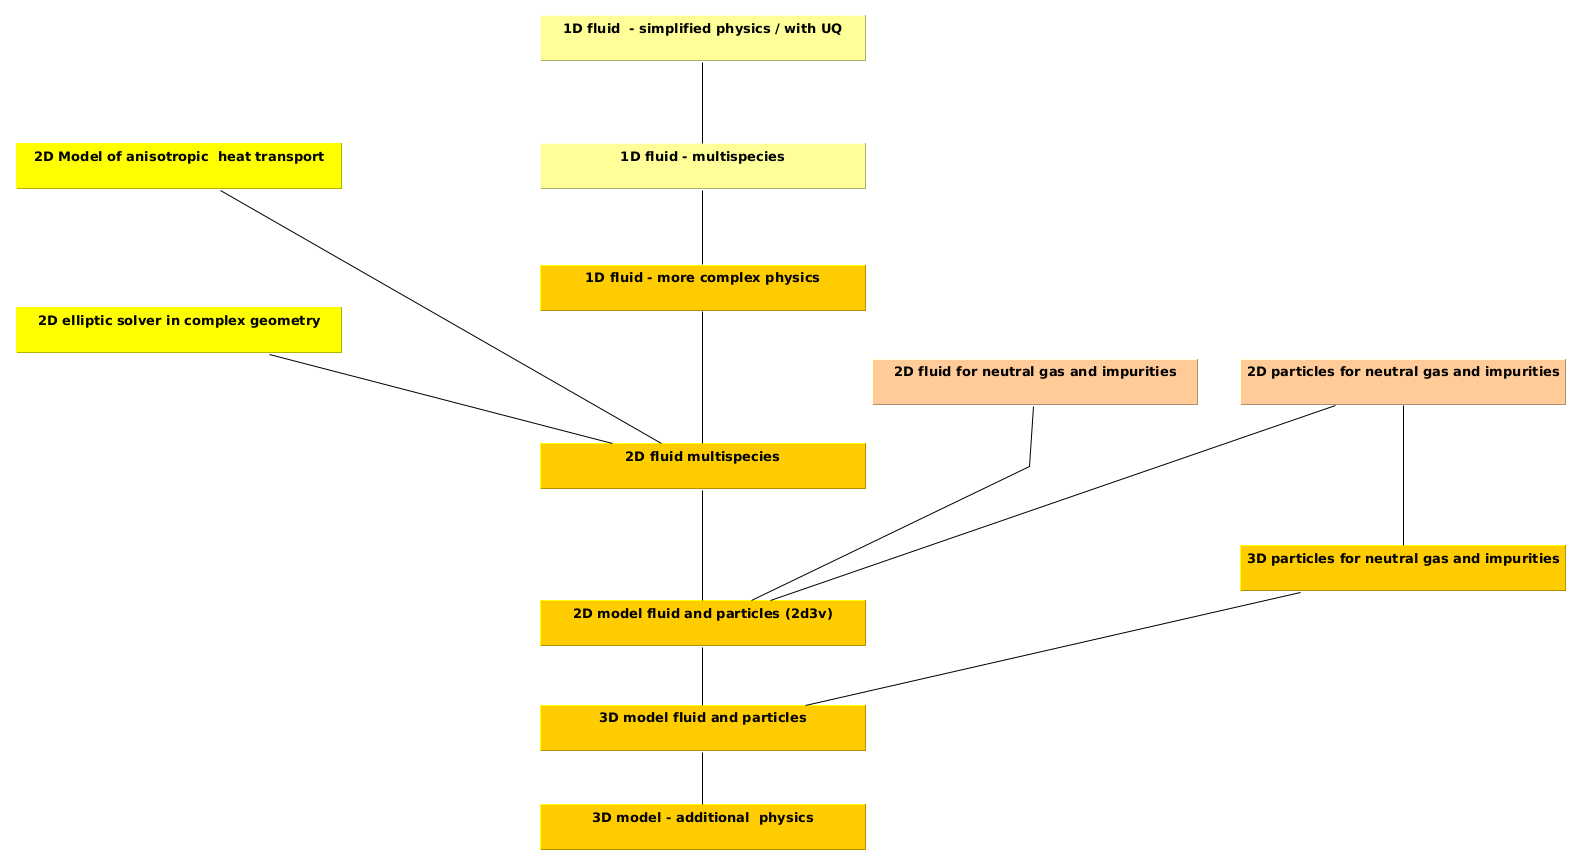
\includegraphics[width=0.95\textwidth]{./pics/proxyflow2.png}}
\caption{
Development of \nep \ software via a sequence of \papp s.
\label{fig:proxyflow2}}
\end{figure}

\subsubsection{Numerical efficiency}

``Numerical efficiency obtained for example through scalability to
large number of cores (given the expected computational resources, the
code should be designed to take: $\sim$1 week for low fidelity
parametric scans; $\lesssim$1 month for medium-high fidelity runs for
advanced design; $\lesssim$3 months for high fidelity physics studies).''

Order of magnitude estimates for the cost of code execution (see~\Sec{cg}),
indicate that these timings are possible but challenging.

The plan is to target Exascale simulations that can support high-fidelity physics
simulations.
Project \nep \ aims to do this in a performance portable fashion using abstraction
layers to separate the physics from the computation details.
However, the challenges of Exascale mean that a degree of
specialisation of the code towards available Exascale machines is expected.
At some point this will probably entail trade-offs that are detrimental to
performance on smaller machines.
Despite this, we still anticipate that the software
should be reasonably performant for small-scale runs.

\subsubsection{Stability of the code}

``Focus on stability of the code, using (preferably) unconditionally
stable numerical schemes and capability to diagnose and re-start failed runs.
Ensure a small failed simulation rate for common configurations.''

The focus will be on accuracy rather than stability.
An accurate solution will be a stable one, whereas the converse is not true.
The use of bifurcation tracking techniques is expected to help with numerical
stability. 
Moreover, the use of ensemble techniques (as part of uncertainty quantification)
should provide information on stability as a function of parameters, as well as
making it likely that at least a subset of calculations produces usable
results.

In addition, there are some planned technical solutions for diagnosing problems
with runs.
The simplest functionality is to allow users to change parameters when
restarting a job using checkpoint files.
The code can also be made to automatically check input files (to catch user
misspellings), and to output a file containing the parameters that were
actually used in a simulation (in case some were accidentally overwritten).
Simulations may also be given a Universally Unique Identifier (UUID) to allow
provenance tracking of simulations.


\subsubsection{Exhaust physics modelling capability}

``Provide capability to model exhaust physics all the way from sheath
limited to strongly detached regimes.''

This capability follows from (1) the implemented physics models/boundary
conditions, and (2) the lengthscales the code can resolve in simulations of
feasible run times.
Project \nep \ anticipates that this will be feasible. 
See \S\ref{sec:physics_model} for further details for the physical
models.


\subsubsection{Modern software design}

``Modern software design with modular approach (independent and efficient libraries).''

Project \nep \ is certainly adopting a modular approach to software design.
This is crucial for enabling many of the desired features, as noted below.
The use of reliable third-party libraries is also vital for enabling a small
team of developers to leverage the work of others, and to allow code
flexibility and ease of prototyping.

\subsubsection{Ability to integrate with other codes (eg.\ with IMAS).}
This feature is anticipated, and will be facilitated by writing the code in
object-oriented C++.

Integration with IMAS (and other data formats/standards) can be achieved by
writing a module to translate between \nep's internal data structures and IMAS
format.
\nep\ developers are involved in TSVV software which will also integrate with
IMAS, so will have experience in this area.

\subsubsection{Modern visualisation tools}
Integration with modern visualisation tools is not specifically addressed in
the science plan.
However, this is enabled by using standard data formats such as netCDF/HDF5.
Auxiliary tools (similar to BOUT++'s xBOUT library) could also be developed.

The issue of \emph{in situ} visualisation will also be important at the Exascale,
with the need to interrogate large quantities of data without moving it,
perhaps during a simulation.
Project \nep \ does not have specific plans for enabling this.
However, the need for this will be widespread, and we expect third-party
tools/libraries to become available to support this, particularly in C++.

\subsubsection{Accessibility (output easily catalogued and interrogated  big data)}
Given the constraint of producing Exascale volumes of data,
it is expected that \nep\ will default to using the Met Office practice of only
saving the files necessary for repeating a simulation, rather than full
outputs.
It is intended that key aspects will be captured by surrogates, descriptions of
which will be saved and indexed.
Users however will be able to choose to output more data and to define
custom diagnostics.
A modular approach to software design and the use of standard libraries will
ease the implementation of these.

In time, there will likely be a move towards creating
simulation databases in preference to repeating expensive simulations.
Such projects are nascent, but we have collaborators who are working in this
area.
Again, the modular approach and use of standard data structures will enable
interfacing with such databases as the technology matures.

% WA: It is expected that we shall adopt Met Office practice and only save the
% files needed to repeat simulations, rather than full outputs. It is intended
% that key aspects will be captured by surrogates, descriptions of which will
% be saved and indexed.
% JTP: Outputting more would be a user option though?

\subsubsection{Version control and user support.}
Version control is a fundamental part of modern software development, and will
certainly be used in \nep.
More generally, the project will use best software practices, including
protected branches, peer reviewed pull requests, issue trackers and automated
testing.
The main code contributors are familiar with such practices; we have heavy
involvement from the projects BOUT++ and Nektar++ which have very high quality
software practices.
Project \nep \ also have involvement from UKAEA RSEs.

User support will be provided through issue trackers, a project Slack channel,
and where relevant, through training sessions.
Project \nep \ anticipates supporting several classes of user, from
those with limited software knowledge,
to users with appreciation of different numerical/algorithm choices,
through to numerical/software specialists who might edit the code on a granular
level.
Support for such a wide range of uses is enabled by a highly modular
separation-of-concerns approach.

